\documentclass[acmtog]{acmart}
% \AtBeginDocument{%
%   \providecommand\BibTeX{{%
%     \normalfont B\kern-0.5em{\scshape i\kern-0.25em b}\kern-0.8em\TeX}}}

% \usepackage{geometry} % see geometry.pdf on how to lay out the page. There's lots.
\usepackage{amsthm}
\usepackage{url}
% \geometry{a4paper} % or letter or a5paper or ... etc
% \geometry{landscape} % rotated page geometry

% See the ``Article customise'' template for come common customisations

\title{Survey of ZK-SNARK}
\author{Yuncong Zhang}
% \authornotemark[1]
% \email{yczhangsjtu@163.com}
% \affiliation{%
%   \institution{Shanghai Jiao Tong University}
%   \streetaddress{Dongchuan Rd. 800}
%   \city{Minhang}
%   \state{Shanghai}
%   \postcode{200240}
% }

\newcommand{\bbG}{\mathbb{G}}
\newcommand{\cA}{\mathcal{A}}
\newcommand{\cD}{\mathcal{D}}
\newcommand{\cL}{\mathcal{L}}
\newcommand{\cR}{\mathcal{R}}
\newcommand{\Setup}{\mathsf{Setup}}
\newcommand{\Prove}{\mathsf{Prove}}
\newcommand{\Verify}{\mathsf{Verify}}
\newcommand{\Comm}{\mathsf{Comm}}
\newcommand{\Open}{\mathsf{Open}}
\newcommand{\Eval}{\mathsf{Eval}}
\newcommand{\pp}{\mathsf{pp}}
\newcommand{\cm}{\mathsf{cm}}
\newcommand{\PiL}{\Pi_{\cL}}
\newcommand{\Ext}{\mathsf{Ext}}
\newcommand{\Sim}{\mathsf{Sim}}
\newcommand{\tr}{\mathsf{tr}}
\newcommand{\polylog}{\mathsf{polylog}}
\newcommand{\poly}{\mathsf{poly}}
% \date{} % delete this line to display the current date

%%% BEGIN DOCUMENT
\begin{document}

% \tableofcontents
% \newpage
\begin{abstract}
\end{abstract}

\maketitle

\section{Introduction}

Zero-Knowledge Succinct Non-interactive ARgument of Knowledge (zkSNARK)~\cite{BitanskyCCT12} enables constant-or-logarithmic-time verification of computation outputs without knowing the inputs.
The zkSNARKs are particularly useful in blockchains~\cite{Ben-SassonCG0MTV14, SunALY17}, where zkSNARKs facilitate creating confidential transactions that conceal part or all of the transaction details.
Currently, zkSNARKs are under active research, and recent years have seen an explosion of zkSNARK constructions enjoying different properties, including constant-size proofs~\cite{Groth16, GennaroGP013, Ben-SassonCGTV13, ParnoHG013, Ben-SassonCTV13}, universal or trustless setups~\cite{GrothKMMM18, MallerBKM19, BunzFS20, Ben-SassonBHR18, Ben-SassonCRSVW19, AmesHIV17}, and post-quantum security~\cite{Ben-SassonBHR18, Ben-SassonCRSVW19}.


However, the rapid development of zkSNARK poses considerable challenges for researchers to keep up with the state-of-the-art.
Existing zkSNARK constructions rely on a large and growing number of underlying tools, examples shown in Table~\ref{tab:build.tool}.
Existing reviews of literature~\cite{ZKProof20, Nitulescu19, WalfishB15} only introduced these tools separately instead of in a unified perspective.
It is also tricky to assess and compare existing schemes due to the high-dimensionality of measurement metrics, summarized in Table~\ref{tab:measure}.
Most of the studies that propose new constructions include an efficiency analysis and compare their products with previous ones.
But these analysis are often incomplete and, to make things worse, diverse in notations, metrics, and parameters.
A comprehensive survey of literature in zkSNARKs can serve as an anchor of knowledge in this field, to enhance understanding of why and how zkSNARKs appeared and thrived, to help selecting appropriate zkSNARKs for different application scenarios, to reveal the insights behind current constructions, and to uncover the full potential of the existing techniques to construct more efficient and secure zkSNARKs.

\begin{table}[tb]
	\caption{Examples of zkSNARK building tools}
	\label{tab:build.tool}
	\centering

	\begin{tabular}{cccc}
	\hline

	\hline
	\textbf{Proof Model} & \textbf{Computation Model} & \textbf{Cryptography}\\
	\hline
		IP~\cite{GoldwasserMR85}       & Boolean circuit                  & Polynomial commitments~\cite{KateZG10} \\
		PCP/PCPP~\cite{BabaiFLS91}     & Arithmetic circuit               & CRH/ECRH \\
		IPCP                           & Structured circuit               & Bilinear pairing~\cite{BonehF01} \\
		IOP/IOPP~\cite{Ben-SassonCS16} & Layered circuit                  & Fiat-Shamir~\cite{FiatS86} \\
		LPCP/LIP~\cite{BitanskyCIPO13} & Random access machine            & Accumulator \\
		                               & QSP/QAP/SSP~\cite{GennaroGP013}  & Multi-party computation \\
		                               & AIR/ACSP~\cite{Ben-SassonBHR18}  & Lattic-based \\
		                               & R1CS                             & Group of unknown order~\cite{BunzFS20} \\
	\hline

	\hline
	\end{tabular}
\end{table}

\begin{table}[tb]
	\caption{Measurement metrics for zkSNARKs}
	\label{tab:measure}
	\centering

	\begin{tabular}{ccc}
	\hline

	\hline
	\textbf{Efficiency} & \textbf{Security} & \textbf{Functionality} \\
	\hline
		Prover complexity & Soundness & Expressiveness  \\
		Verifier complexity & Zero-knowledgeness & Public verifiability \\
		Setup complexity & Trusted setup & Universality \\
		Proof length & Post-quantum security & (Non)Preprocessing \\
		CRS length & Cryptographic assumption & \\
	\hline

	\hline
	\end{tabular}
\end{table}

In this paper, we present a survey that summarizes the knowledge of zkSNARKs in a systematic way.
To begin the story, we recall the history of zkSNARKs to undertsand the role zkSNARK plays in a broader field called ``proof systems''.
For the most part of this survey, we present the knowledge of zkSNARKs in three levels:
\begin{enumerate}
	\item In the theoretical level, we provide a definition for zkSNARK as a special case of proof systems.
	Based on this definition, we illustrate current theoretic results on zkSNARKs, e.g. the best efficiency we can achieve under certain security assumptions.
	\item In the technical level, we review and unify the existing frameworks of zkSNARK constructions.
	In this unified framework, we classify and examine the existing zkSNARKs to reveal the insights behind the construction techniques.
	\item In the application level, we propose an analysis system for measuring and comparing zkSNARKs.
	Instead of the traditional way that emphasizes the asymptotic complexities and practical performance in ``toy examples'', our system focus on evaluating the practicality of zkSNARKs in different application scenarios.
	Using this system, we conduct a comprehensive comparison of existing constructions.
\end{enumerate}

\section{Related Works}



\section{Preliminaries}

Designing zkSNARKs requires systematic use of cryptography and computational complexity theory.
We will illustrate the concepts in these fields that are most relevant to zkSNARKs.

\subsection{Notations}

We use $\cR$ for an NP relationship, i.e. a set of pairs $\{(x,w):f(x,w)=0\}$ where $x$, $w$ are bit strings of size $n$ and $f$ is a deterministic polynomial-time algorithm.
The NP language $\cL$ induced from $\cR$ is the set $\{x:\exists (x,w)\in\cR\}$.
For $(x,w)\in\cR$, we say $x$ is an instance of $\cL$ and string $w$ is a witness of the fact $x\in\cL$.

We say a system has $\lambda$-bit security if breaking this system costs at least $2^{\lambda}$ units of computation power.
We use $n$ for the bit-lengths of algorithms inputs.
We use $\eta(n)$ for a negligible function in $n$, $\polylog(n)$ for a poly-logarithmic function, and $\poly(n)$ for a polynomial function.
We say an algorithm is p.p.t. if the algorithm is probabilistic and can only execute for a period of length $\poly(n)$.

\subsection{Proof systems}

A proof system is a protocol that allows a party, namely the prover, to prove a statement to another party, namely the verifier.

\paragraph{Statements.} Proof systems usually deal with two types of statements related to an NP language $\cL$:
\begin{enumerate}
	\item given string $x$, the statement claims that $x\in\cL$;
	\item given string $x$, the statement claims knowledge of $w$ such that $(x,w)\in\cR$.
\end{enumerate}

\paragraph{Syntax.}
Given an NP language $\cL$, a proof system $\PiL$ consists of three algorithms $(\Setup,\Prove,\Verify)$.
\begin{enumerate}
	\item $\Setup(\pp)\to(\sigma_P,\sigma_V)$. The $\Setup$ algorithm takes public parameters $\pp$ as inputs and generates reference strings $\sigma_P$ and $\sigma_V$ for the prover and the verifier respectively.
	The reference strings $\sigma_P$ and $\sigma_V$ may intersect with each other, in which case, the intersection is called a \emph{common reference string (CRS)}.
	The $\Setup$ algorithm must be executed before any instance of $\Pi$ can start.
	\item $\langle\Prove(\sigma_P, x, w)\rightleftharpoons\Verify(\sigma_V, x)\rangle\to 0/1$.
	Given a pair $(x,w)\in\cR$, the $\Prove$ algorithm takes a pair $(x,w)$ and the reference string $\sigma_P$ as inputs.
	The $\Verify$ algorithm takes $x$ and the reference string $\sigma_V$ as inputs.
	When being executed, the algorithms may exchange messages between each other.
	Finally, the $\Verify$ algorithm outputs 0 or 1, which is regarded as the output of this protocol.
\end{enumerate}
The execution of a proof system is illustrated in Fig.~\ref{fig:proof.system}.
\begin{figure}[ht!]
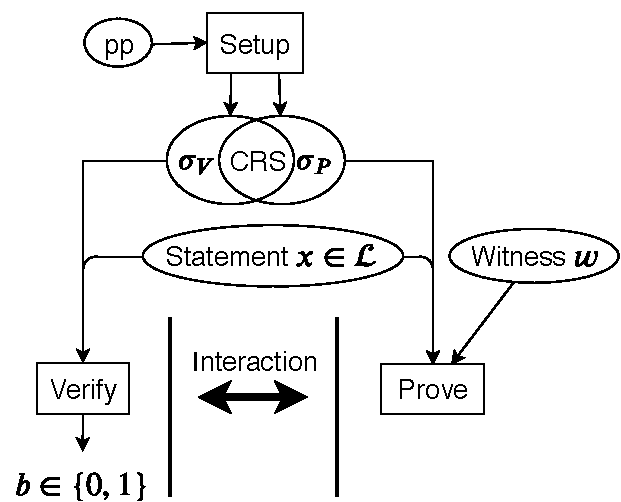
\includegraphics[width=0.3\textwidth]{images/proof-system.pdf}
\caption{Proof System}
\label{fig:proof.system}
\descriptionlabel{An example of a proof system execution.
The rectangles represent algorithms.
The ovals represent inputs to these algorithms.}
\Description{}
\end{figure}


\paragraph{Properties.}
A proof system $\PiL=(\Setup,\Prove,\Verify)$ is expected to satisfy the following properties:

\begin{definition}[Completeness]
\label{def:completeness}
A proof system $\PiL=(\Setup,\Prove,\Verify)$ has \emph{completeness} if for any $(x,w)\in\cR$, correctly executing the protocol always outputs $1$, i.e.
	\begin{eqnarray}
	\Pr\left[b=1\left|
	\begin{matrix}
	\Setup(\pp)\to(\sigma_P,\sigma_V);\\
	\langle\Prove(\sigma_P, x, w)\rightleftharpoons\Verify(\sigma_V, x)\rangle\to b
	\end{matrix}
	\right.\right]=1
	\end{eqnarray}
\end{definition}

\begin{definition}[Soundness]
\label{def:soundness}
	A proof system $\PiL=(\Setup,\Prove,\Verify)$ has \emph{soundness} if for any $x\notin\cL$, for any adversary $\cA$ acting as the prover, the protocol outputs $1$ with probability $\epsilon < 1/2$, where $\epsilon$ is called the soundness error of $\PiL$.
	\begin{eqnarray}
	\label{eqn:soundness}
	\Pr\left[b=1\left|
	\begin{matrix}
	\Setup(\pp)\to(\sigma_P,\sigma_V);\\
	\langle\cA(\sigma_P, x)\rightleftharpoons\Verify(\sigma_V, x)\rangle\to b
	\end{matrix}
	\right.\right]=\epsilon < 1/2\,
	\end{eqnarray}
	If equation (\ref{eqn:soundness}) holds only for p.p.t. adversaries $\cA$, we say $\PiL$ has \emph{computational soundness}.
	In this case, we say $\PiL$ is an \emph{argument system}.
\end{definition}

Note that given $\PiL$ with non-negligible soundness error $\epsilon < 1/2$, we can always construct $\PiL'$ with exponentially small soundness error $\epsilon'$, by repeating the protocol a polynomial number of times.
Therefore, requiring the soundness error to be smaller than $1/2$ is sufficient for a proof system to be useful in practice.

\paragraph{Variations.}
Based on the standard definitions described above, proof systems may take variations in many aspects.
\begin{enumerate}
	\item \emph{Proof-of-knowledge.} Informally, a proof system is said to have proof-of-knowledge, if Definition~\ref{def:soundness} holds not only for $x\notin\cL$, but also for $x\in\cL$ if the adversary does not ``know'' any witness of $x$.
	The notion ``knowledge'' is formally defined by an extractor algorithm.
	\begin{definition}[Proof-of-Knowledge]
	\label{def:proof.of.knowledge}
	A proof system $\PiL=(\Setup,\Prove,\Verify)$ has \emph{proof-of-knowledge} if for any $x\in\{0,1\}^n$, for any adversary $\cA$ acting as the prover, there exists a negligible function $\eta(n)$ and an extractor $\Ext^{\cA}$ which has non-blackbox access to the adversary, such that whenever the adversary successfully cheats the verifier into outputing $1$, $\Ext^{\cA}$ outputs a witness $w$ s.t. $(x,w)\in\cR$ with overwhelming probability, i.e.
	\begin{eqnarray}
	\label{eqn:proof.of.knowledge}
	\Pr\left[
		\begin{matrix}
		b=1\wedge \\
		(x,w)\notin\cR
		\end{matrix}
	\left|
		\begin{matrix}
		\Setup(\pp)\to(\sigma_P,\sigma_V);\\
		\langle\cA(\sigma_P, x)\rightleftharpoons\Verify(\sigma_V, x)\rangle\to b;\\
		\Ext^{\cA}(\sigma_P, x)\to w
		\end{matrix}
	\right.\right]=\eta(n)\,
	\end{eqnarray}
	If equation (\ref{eqn:proof.of.knowledge}) only holds for computationally bounded adversaries, we say the proof system has \emph{argument-of-knowledge}.
	\end{definition}

	\item \emph{Zero-knowledge.} A proof system is said to be zero-knowledge if the verifier cannot extract any ``knowledge'' from the interaction transcripts, i.e. the collection of all the messages sent during the protocol execution.
	The zero-knowledge property is formally defined by a simulator algorithm.
	\begin{definition}[Zero-knowledgeness]
	\label{def:zero.knowledge}
	Let $\tr=[\Prove(\sigma_P, x)\rightleftharpoons\Verify(\sigma_V, x)]$ be the interaction transcript between the prover and the verifier, and call $(\sigma_V,\tr)$ the view of the verifier.
	A proof system $\PiL=(\Setup,\Prove,\Verify)$ is zero-knowledge if for any adversary $\cA$ acting as the verifier, there exists a simulator $\Sim(\cdot)$ such that for any $(x,w)\in\cR$, $\Sim(x)$ is indifferentiable from the view of $\cA$ during the protocol execution, i.e. there exists negligible function $\eta(n)$, s.t. for any differentiator $\cD$:
	\begin{eqnarray}
	\label{eqn:zero.knowledge}
	\left|
	\begin{matrix}
	\Pr\left[
		\begin{matrix}
		\cD(\sigma_V,tr)=1
		\end{matrix}
	\left|
		\begin{matrix}
		\Setup(\pp)\to(\sigma_P,\sigma_V);\\
		[\Prove(\sigma_P, x)\rightleftharpoons\cA(\sigma_V, x)]\to \tr
		\end{matrix}
	\right.\right]\\\\
	-\Pr\left[
		\begin{matrix}
		\cD(\sigma_V,tr)=1
		\end{matrix}
	\left|
		\begin{matrix}
		\Sim(x)\to(\sigma_V,tr)
		\end{matrix}
	\right.\right]
	\end{matrix}
	\right|=\eta(n)
	\end{eqnarray}

	\end{definition}
	The definition of zero-knowledge has some variations.
	\emph{Honest-verifier zero-knowledge} ...
	\emph{Unconditional zero-knowledge} or \emph{perfect zero-knowledge} ...
	\emph{Statistical zero-knowledge} ...
	\emph{Computational zero-knowledge} ...

	\item \emph{Interaction models.} A standard proof system only admits normal interactions, i.e. the prover and the verifier send messages to each other, and each message is read in the whole by the receiver...

	\emph{Non-interactive} ...
	\emph{Probabilistically Checkable Proof (PCP)} ...
	\emph{Interactive PCP (IPCP)} ...
	\emph{Linear PCP (LPCP)} ...
	\emph{Interactive Oracle Proof (IOP)} ...

\end{enumerate}

\emph{Efficiency.} The efficiency of a proof system is measured by the efficiency of each of the algorithms $(\Setup,\Prove,\Verify)$, sizes of the reference strings $(\sigma_P,\sigma_V)$, and the communication cost...

\begin{definition}[Succinctness]
\label{def:succinctness}
A proof system $\PiL$ is succinct if...
\end{definition}

\begin{definition}[Scalability]
\label{def:scalability}
A proof system $\PiL$ is scalable if...
\end{definition}

\subsection{zkSNARK}

With the above definitions on proof systems and their properties, we can now give the definition of zkSNARKs.

\begin{definition}[zkSNARK]
A \emph{zkSNARK} is a proof system that is zero-knowledge (Definition~\ref{def:zero.knowledge}), succinct (Definition~\ref{def:succinctness}), non-interactive, and argument-of-knowledge (Definition~\ref{def:proof.of.knowledge}).
\end{definition}

Depending on how $\Setup$ works, a zkSNARK may be in one or more of the following models.

\paragraph{Preprocessing.} A zkSNARK is called \emph{preprocessing} if ...

\paragraph{Universal setup.} A zkSNARK has \emph{universal setup} if ...

\paragraph{Transparent setup.} A zkSNARK has \emph{transparent setup} if ...

% Fig.~\ref{fig:pp.zksnark} illustrates how preprocessing zkSNARK works.
% \begin{figure}[ht!]
% 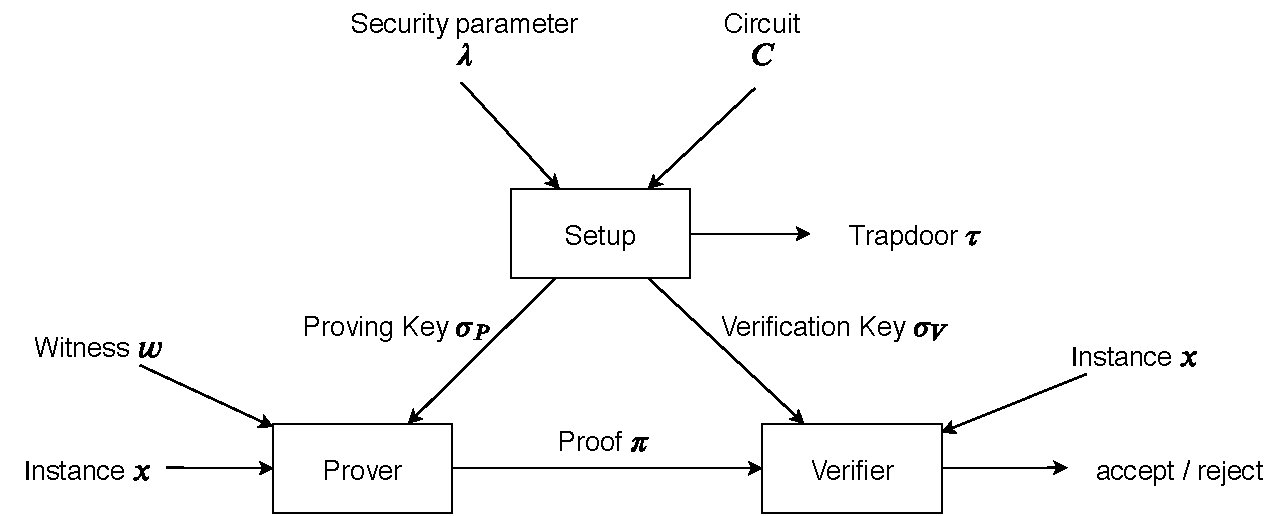
\includegraphics[width=0.4\textwidth]{images/ppzksnark.pdf}
% \caption{Preprocessing zkSNARK}
% \label{fig:pp.zksnark}
% \descriptionlabel{
% The $\Setup$ algorithm takes as inputs both the security parameter $\lambda$ and a circuit $C$, and outputs common reference strings, i.e. the proving key $\sigma_P$ and the verification key $\sigma_V$, to the prover and verifier respectively.
% $\Setup$ also outputs a trapdoor $\tau$ which enables simulating proofs without witness.
% The $\Prove$ algorithm takes as inputs an instance $x$ with corresponding witness $w$, together with proving key $\sigma_P$, and outputs the proof $\pi$ as validation of $x$.
% The $\Verify$ algorithm verifies the correctness of $x$ with proof $\pi$ and verification key $\sigma_V$, and decides if to accept or reject.}
% \Description{}
% \end{figure}

\subsection{Cryptography}

All the existing zkSNARKs are obtained by applying a cryptographic transformation to an information-theoretic proof system~\cite{ZKProof20}.
We will introduce the necessary cryptographic tools behind the major contributions to zkSNARKs.

\paragraph{Commitment scheme.}
A cryptographic commitment scheme enables ...
A commitment scheme is a tuple $\Gamma=(\Setup, \Comm, \Open)$ of p.p.t. algorithms.
\begin{enumerate}
	\item $\Setup(1^{\lambda})\to\pp$ generates public parameters given the security bit number
	\item $\Comm(\pp,m)\to(\cm,r)$ takes a message $m$ and generates a commitment $\cm$, together with an opening hint $r$
	\item $\Open(\pp,\cm,m,r)\to b\in\{0,1\}$ takes a message $m$, a commitment $\cm$ and an opening hint $r$, and verifies if $\cm$ is a valid commitment of $m$.
	If $b=1$, we say $(m,r)$ is a correct opening of $\cm$.
\end{enumerate}
A commitment scheme is expected to be \emph{binding}.

\begin{definition}[Binding]
A commitment scheme $\Gamma=(\Setup,\Comm,\Open)$ is binding if ...
\end{definition}

A commitment scheme can optionally be \emph{hiding}.

\begin{definition}[Hiding]
A commitment scheme $\Gamma=(\Setup,\Comm,\Open)$ is hiding if ...
\end{definition}

\paragraph{Polynomial commitment.} Polynomial commitment schemes are variants of commitment schemes that have message space $R[X]$, i.e. polynomials over ring $R$, and allow opening a single evaluation of the commited polynomial~\cite{KateZG10}.
A polynomial commitment scheme is a tuple $\Gamma=(\Setup,\Comm,\Open,\Eval)$ where $(\Setup,\Comm,\Open)$ is a commitment scheme and $\Eval(\pp,\cm,x,y,d)\to b\in\{0,1\}$ is a protocol ...
Except the binding and hiding properties, a polynomial commitment scheme $\Gamma$ is also expected to be \emph{correct} and \emph{evaluation binding}.

\begin{definition}[Correct]
A polynomial commitment sheme $\Gamma=(\Setup,\Comm,\Open,\Eval)$ is correct if ...
\end{definition}

\begin{definition}[Evaluation binding]
A polynomial commitment sheme $\Gamma=(\Setup,\Comm,\Open,\Eval)$ is evaluation binding if ...
\end{definition}

Sometimes we need a stronger property than the evaluation binding called \emph{knowledge soundness} that requires the prover to ``know'' the committed polynomial~\cite{BunzFS20}.

\begin{definition}[Knowledge soundness]
A polynomial commitment sheme $\Gamma=(\Setup,\Comm,\Open,\Eval)$ has knowledge soundness if ...
\end{definition}

\paragraph{Accumulator.}
Accumulators are another kind of variations of commitment schemes.
Instead of commiting a single element, an accumulator allows commiting to a list of elements, and ...

Merkle-tree is an example of accumulator ...

\paragraph{Fiat-Shamir transformation and random oracle.}
Fiat-Shamir transformation is the standard way to transform a public-coin interactive protocol to a non-interactive scheme.
The Fiat-Shamir transformation works by simulating the verifier challenges by the hash value of prover messages.
However, the security of the resulting non-interactive scheme is established only in the random oracle model.
Current security proving techniques require modeling the hash function by a random oracle, which is an ideal functionality that does not exist in reality.

A random oracle is ...

\paragraph{Bilinear pairing.}
Given groups $\bbG_1$, $\bbG_2$ and $\bbG_T$, with $|\bbG_1|=|\bbG_2|=|\bbG_T|=q$, a bilinear pairing~\cite{BonehF01} is a mapping $e:\bbG_1\times\bbG_2\to\bbG_T$ that satisfies...

\section{zkSNARK Construction Paradigms}

Having learned about the definitions and the building tools, we are ready to investigate the details of current constructions.
As mentioned above,

\section{PCP-based zkSNARKs}

\section{Pairing-based zkSNARKs}

\section{GKR-based zkSNARKs}

\section{MPC-based zkSNARKs}

\section{Comparison of zkSNARKs}

\subsection{Efficiency}

In evaluating the efficiency of zkSNAKRs, the properties we care most about are proving time, verification time, proof sizes, and common reference string sizes.
Fig.~\ref{fig:snark.sizes} summarizes the asymptotic complexities of current zkSNARK implementations.
\begin{figure}[ht!]
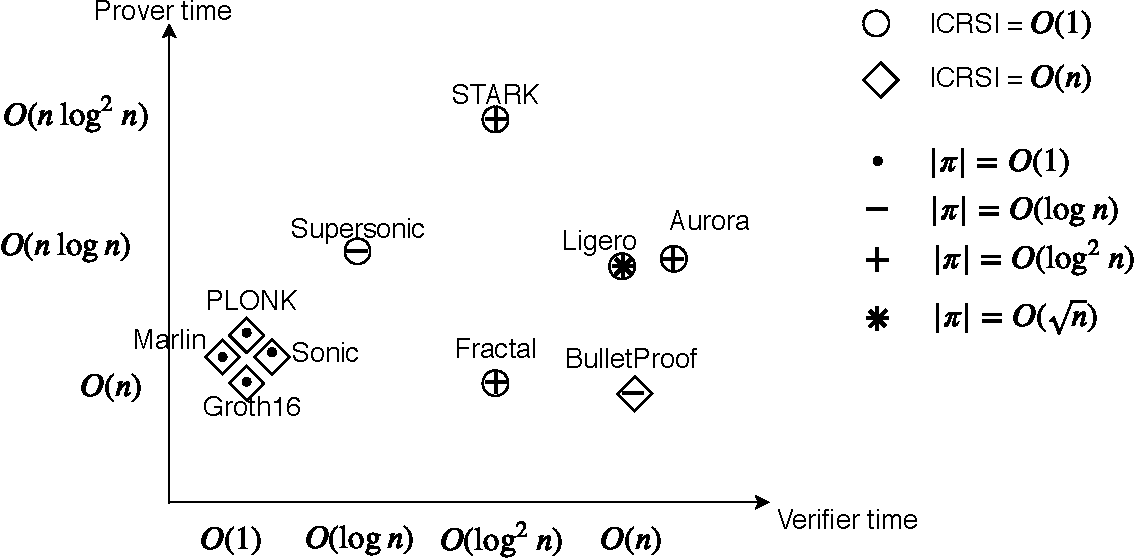
\includegraphics[width=0.4\textwidth]{images/snark-sizes.pdf}
\caption{Asymptotic complexities of zkSNARK implementations}
\label{fig:snark.sizes}
\descriptionlabel{
The big-$O$ notation here hides the security parameter $\lambda$.
The $n$ denotes the statement size.
For circuit-based zkSNARKs, $n$ is the circuit size.
For statements with succinct representation, e.g. STARK, $n$ is the length of execution trace, i.e. the size of the circuit representing the unrolled computation.}
\Description{}
\end{figure}

\subsection{Security}

\subsection{Functionality}

\section{Conclusion}

\bibliographystyle{unsrt}
\bibliography{reference}

\end{document}